\section{Setup}
\label{sec:setup}
% (1 page)

% TODO: move to a figure.
%``[Carrie] Fisher’s mother, entertainer Debbie Reynolds, said on Twitter on Sunday that her daughter was in stable condition.''
%Teams are then required to identify spans in the text that correspond to entities (e.g. ``\textit{Fisher}'', ``\textit{Debbie Reynolds}''),
%assign these entities a canonical id (e.g. \texttt{Carrie\_Fisher}, \texttt{Debbie\_Reynolds})
%  and, finally, identify all facts about mentioned entity expressed in the surrounding context (e.g. \texttt{Carrie\_Fisher per:parents Debbie\_Reynolds} or \texttt{Debbie\_Reynolds per:title entertainer}).

\begin{figure*}[ht]
  \centering
  \begin{subfigure}{0.49\textwidth}
    % TODO: example figure.
  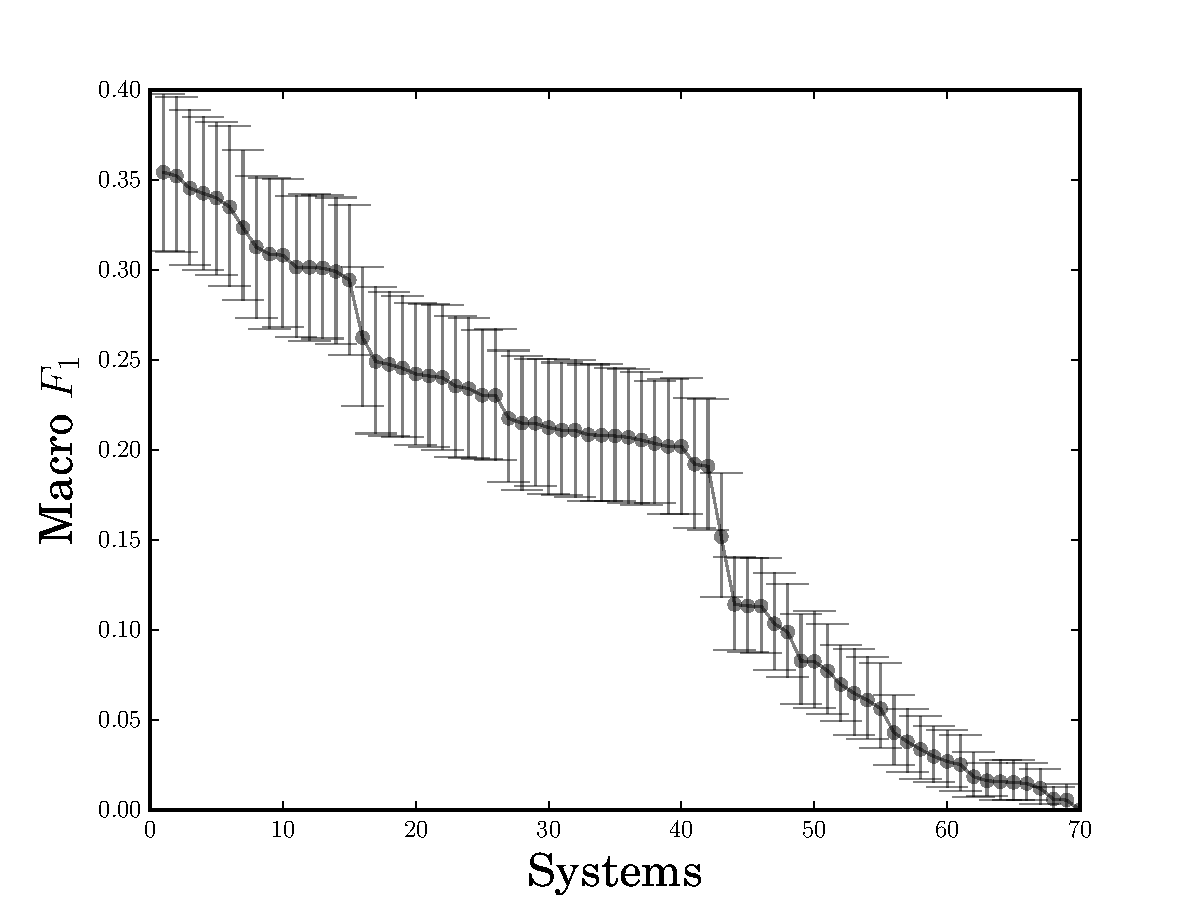
\includegraphics[width=\columnwidth]{figures/experiment1}
  \end{subfigure}
  \hfill
  \begin{subfigure}{0.49\textwidth}
  % vim:ft=tex
% Diagram depciting how mentions and entities are sampled.
\documentclass{article}
%\usetikzlibrary{...}% tikz package already loaded by 'tikz' option
\usepackage{scabby-diag}
\usepackage{booktabs}
\usetikzlibrary{fit}
\usetikzlibrary{patterns}

\begin{document}

\tikzset{correct/.style = {fill=green},
         incorrect/.style = {pattern=north east lines, pattern color=red},
         node/.style = {circle, scale=.7},
         sysa/.style = {draw, circle, dashed, thick, purple},
         sysb/.style = {draw, circle, dotted, thick, blue},
         output/.style = {inner sep=-2pt},
         duplicate/.style = {draw, rectangle, thick, red},
         part/.style = {draw, rectangle, dashed, black, thick},
        }

\begin{table}
\begin{tabular}{l | c c c c} \toprule
  $s$ & $f_1$ & $f_2$ & $f_3$ & $f_4$ \\ \midrule
  & 
    \tikz{
  \node[node,correct] (m11){$m_{11}$};
  \node[sysa,output,fit= (m11)] (m11A){};
  } 
  & 
  \tikz{
  \node[node, correct] (m21) {$m_{21}$};
    \node[sysa, output, fit= (m21)] (m21A) {};
  }
  & 
  \tikz{
    \node[node, correct] (m31) {$m_{31}$};
    \node[sysa, output, fit= (m31)] (m31A) {};
    }
  & 
  \tikz{
    \node[node, correct] (m41) {$m_{41}$};
    }
  \\

  & 
  \tikz{
  \node[node,incorrect] (m12){$m_{12}$};
  \node[sysb,output,fit= (m11)](m11B){};
  } 
  & 
  \tikz{
    \node[node, incorrect] (m22) {$m_{22}$};
    \node[sysb, output, fit= (m22)] (m22B) {};
  }
  
  &
  \tikz{
    \node[node, correct] (m32) {$m_{32}$};
    \node[sysa, output, fit= (m32)] (m32A) {};
    \node[duplicate, fit= (m32A)] (m32AD) {};
    }
  & \\
  & 
  \tikz{
    \node[node,correct] (m13){$m_{13}$};
  }
  & & & \\
  & 
    \tikz{
  \node[node,correct] (m14){$m_{14}$};
  \node[sysa,output,fit= (m14)] (m14A){};
  \node[sysb,output,fit= (m14A)]{};
  } 
  \\
  \bottomrule

\end{tabular}
\end{table}


\end{document}

  \end{subfigure}
  \caption{Evaluating KBP}
\end{figure*}

In the knowledge base population task, 
 you are given a document corpus $D$, typically containing 10,000--100,000 documents,
 and must return a list of all the entities and relations\footnote{
 We consider only binary relations in this work.
 } contained in the corpus.

Let's consider the example in \figureref{example} about the late actress Carrie Fisher to understand how entities and relations are specified. 
This sentence mentions three entities,
  ``\textit{Fisher}'',
  ``\textit{Debbie Reynolds}'',
  ``\textit{Twitter}''.
We will use $m$ to refer to a mention (e.g.\ ``\textit{Fisher}''), which is simply a span of text in a document, and $e$ to refer to the entity described by that mention (e.g.\ \texttt{Carrie\_Fisher}).
The sentence describes a relation $r$, \texttt{per:parents}, between the mentions $m_s$, ``\textit{Fisher}'', and $m_o$ ``\textit{Debbie Reynolds}'', and consequently a relation between the entities \texttt{Carrie\_Fisher} and \texttt{Debbie\_Reynolds}.
We will use $f$ to refer to the pair ($r$, $e_o$), sometimes referred to as a ``slot fill''.
Finally, when returning entity mentions and relations, the surrounding context $c$ used to justify the link or relation must also be specified.

As you can see, knowledge base population is actually composed of three tasks: entity detection, entity linking and relation extraction.
This coupling allows us to aggregate facts extracted from multiple documents by the canonical entity and ask relational queries of the database so constructed, e.g.\ ``what do Carrie Fisher's parents do?''
Accordingly, evaluating the output of a KBP system can be defined at two levels, at the mention-level and at the entity-level.
Let us now see an example of how to score the output of two systems $A$ and $B$, summarized in \figureref{evaluation-table}.

At the mention-level, we only evaluate a system as correctly identified whether two mentions $m_s$ and $m_o$ share a relation $r$ \textit{given the context $c$}, irrespective of bad linking decisions (e.g.\ linking the \textit{Fisher} in the text with the mathematician \texttt{Ronald\_Fisher}).
In this example, we can compute the \textit{mention-level} precision and recall as,
\begin{align*}
  P^m_A &\eqdef \frac{|C \intersection C^*|}{|C|} = \frac{|\{c_{11}, c_{14}, c_{21}, c_{31}, c_{32}\}|}{|\{c_{11}, c_{14}, c_{21}, c_{31}, c_{32}\}|} = 1 \\
  R^m_A &\eqdef \frac{|C \intersection C^*|}{|C^*|}\\
  &= \frac{|\{c_{11}, c_{14}, c_{21}, c_{31}, c_{32}\}|}{|\{c_{11}, c_{14}, c_{21}, c_{31}, c_{32}, c_{13}, {c_{41}}\}|} = \frac{5}{7},
\end{align*}
where $C$ is the set of all contexts predicted to contain relation returned by the system and $C^*$ are the set of all contexts that contain a relation in the corpus.

At the entity-level, we focus on an entity $e_s$ and ask if the system has correctly identified a relation $r$ with another entity $e_o$ \textit{given some context $c$}, or the fill $f$.
Thus, system's A and B both get full credit for identifying the fill $f_1$, even though system A had found two contexts that expressed $f_1$.  
On the other hand, if a system falsely reports two distinct fills when there was only one, as was the case with system A and $m_{32}$, only one is considered correct, and the system loses precision for reporting an incorrect answer. 
Thus, the entity-level precision and recall scores are,
\begin{align*}
  P^e_A &\eqdef \frac{|F \intersection F^*|}{|F|} &= \frac{|\{f_{1}, f_{2}, f_{3}\}|}{|\{f_{1}, f_{2}, f_{3}, f_{3}'\}|} &= \frac{3}{4} \\
  R^e_A &\eqdef \frac{|F \intersection F^*|}{|F^*|} &= \frac{|\{f_{1}, f_{2}, f_{3}\}|}{|\{f_{1}, f_{2}, f_{3}, f_{4}\}|} &= \frac{3}{4}.
\end{align*}
where $F$ is the set of all slot fills for the entity $e$ returned by the system and $F^*$ are the set of all slot fills for the entity $e$ in the corpus.

The entity-level metrics can be either micro or macro averaged.
% TODO: fix notation. handle \fone.
The standard metric we will be using in this paper is macro-averaged $\fone^e \eqdef \frac{1}{|E|} \sum_{e \in E} \fone^{e}$.

\paragraph{The TAC-KBP competition.}
% TODO provide some details about the competition -- its history. Talk about how slotfilling led to kbc.
%

\paragraph{Evaluation methodology.}
% TODO how is the output evaluated? what are queries (how many)? how much output is evaluated? Human systems? what metrics are used (in relation to math above). Quick note about entry points and how entities are identified as being the same cluster / id as a specified entity.

